\newpage 

\subsection{Use case diagram}
\label{subsec:useCaseDiagram}
Figur \ref{fig:UCD} viser de identificerede use cases.
\vspace{-10pt}
%Usecase diagram indføres i følgende 5 linjer, derefter starter UC 1
\begin{figure}[H]
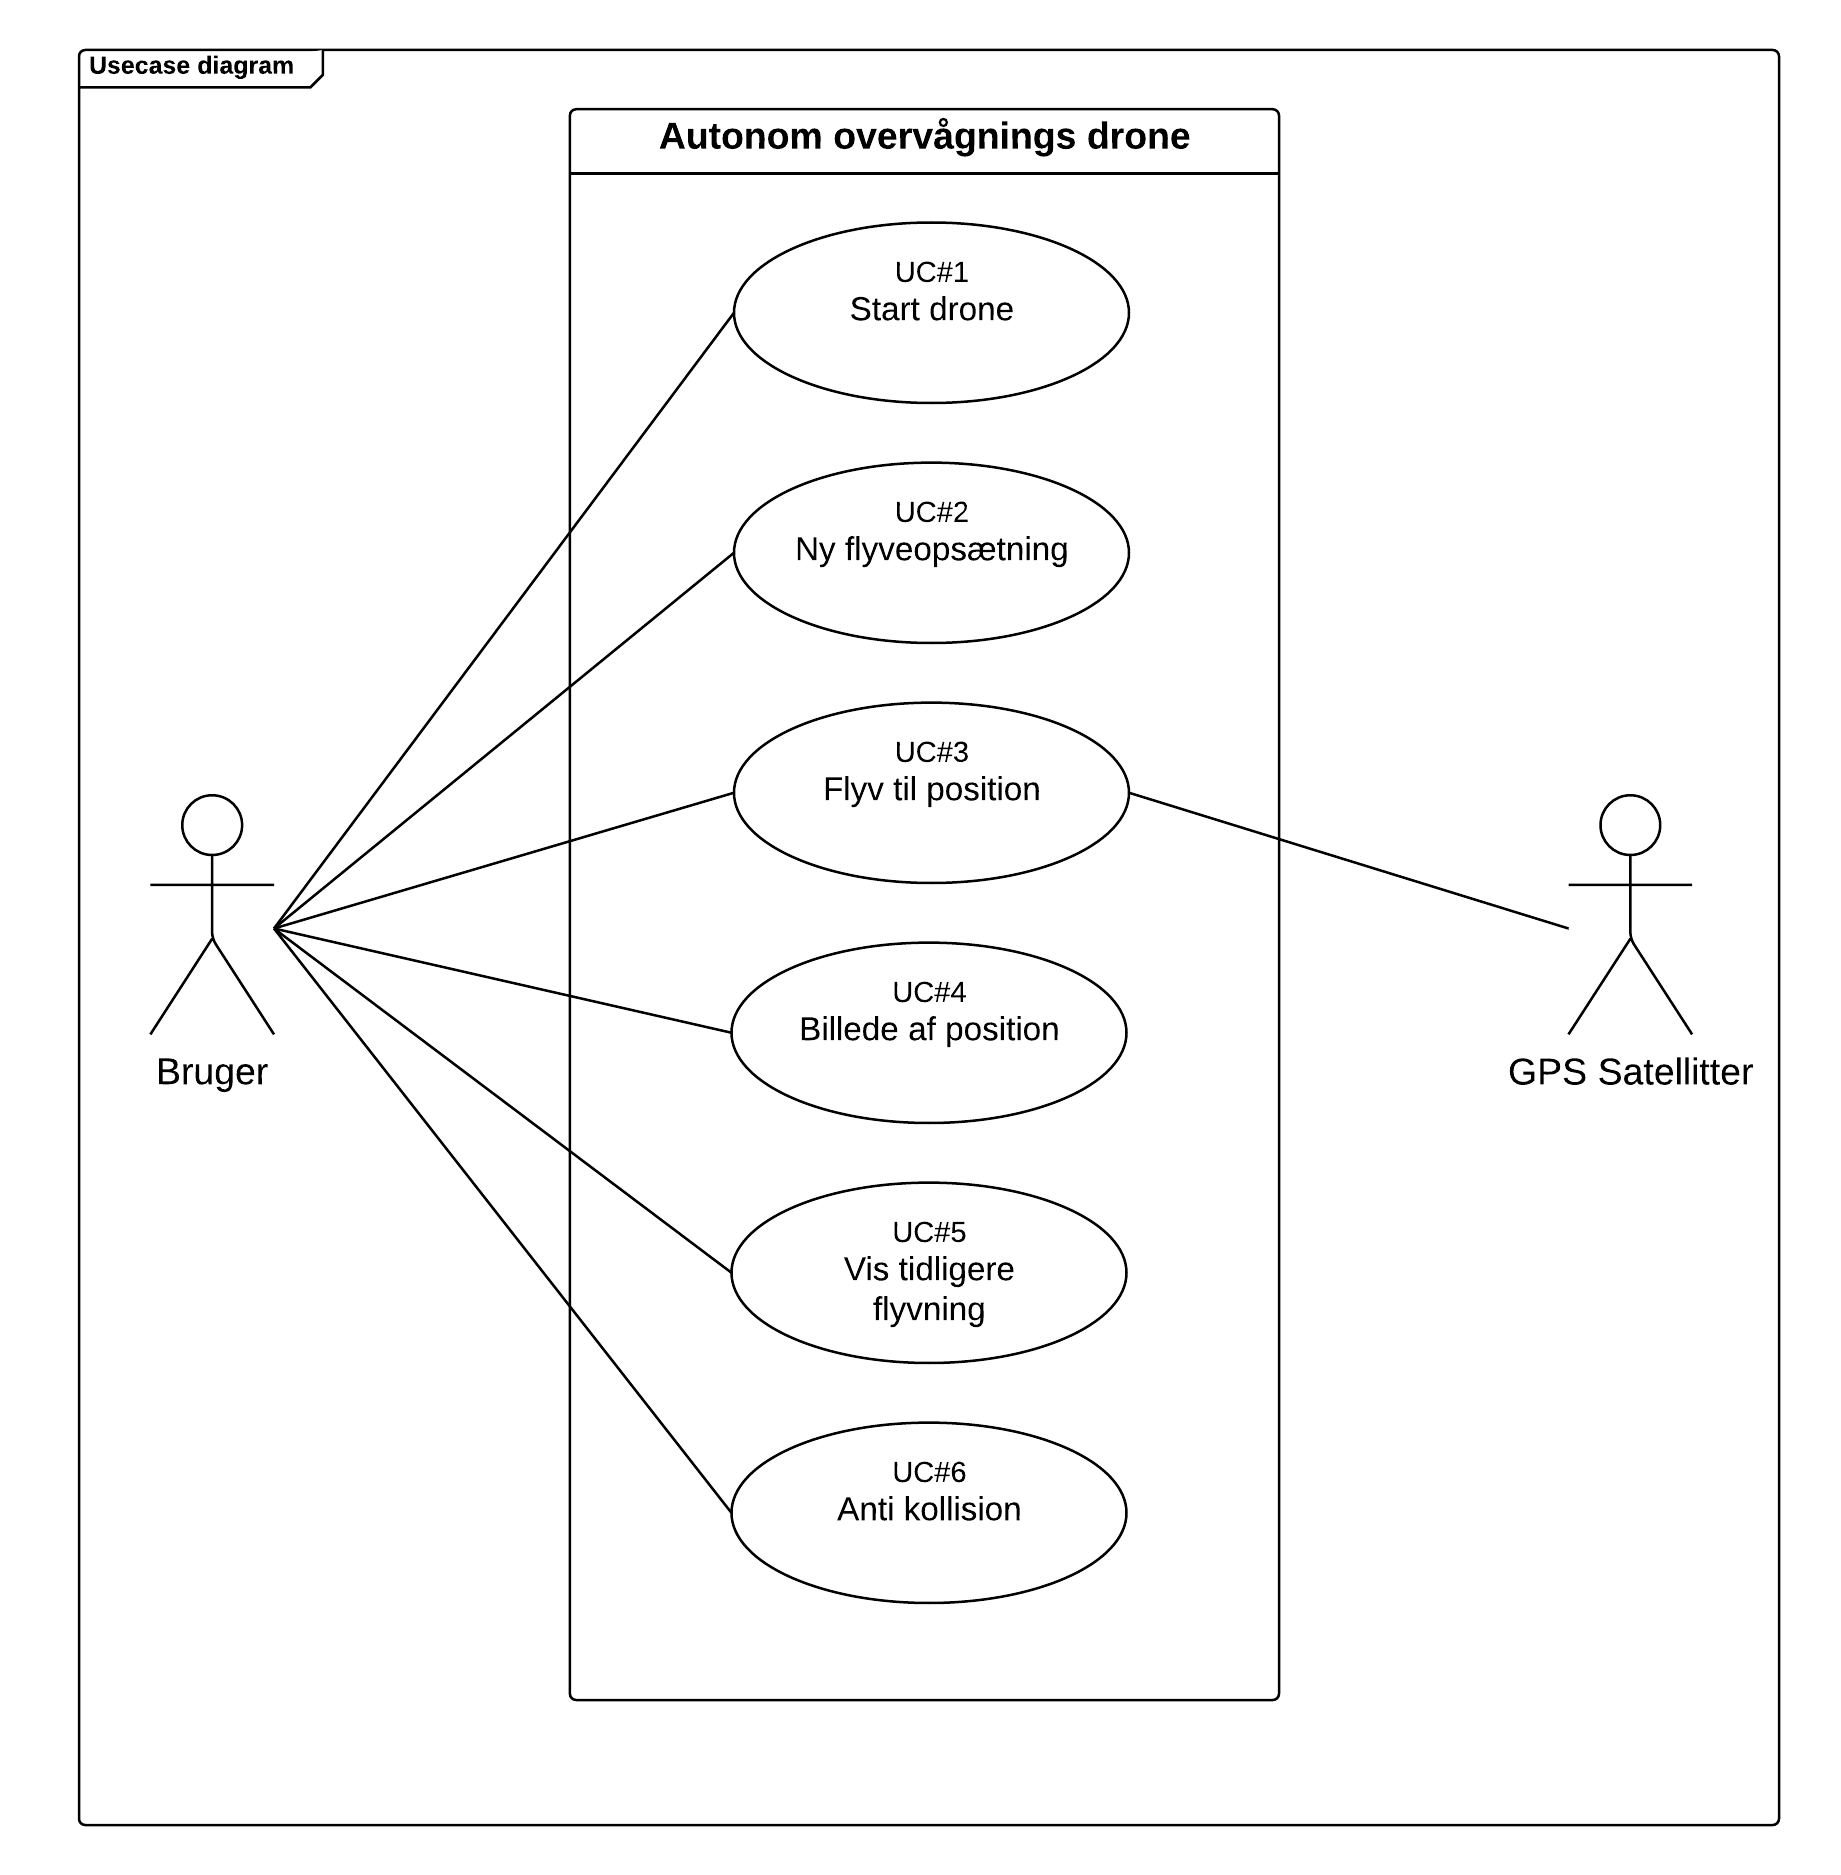
\includegraphics[width=1\textwidth]{Billeder/Use_case_diagram.png}
\vspace{-0.8cm}
\caption{Use case diagram}
\label{fig:UCD}
\end{figure}




\newpage
\subsection{Udviklingsforløb}

For at gøre udviklingsforløbet mere overskueligt gøres brug af iterationer.
De iterationer der ligger tidligst i udviklingsforløbet er mest essentielle for systemet, 
mens de iterationer der ligger senere i forløbet prioriteres knap så højt.
Udviklingsforløbet i dette projekt er planlagt til at forløbe via 4 iterationer. Nedenfor beskrives hvad der skal laves i de forskellige iterationer. \\

\textbf{Iteration 1:} \\
I denne iteration tages hånd om systemet mest grundlæggende funktionalitet. Batteri, ESC'er, motorer og ultralyds sensorer tilsluttes dronen. Desuden gøres dronen i stand til at kunne oprette forbindelse til internettet via 3G-shield. Når iteration 1 er færdig skal UC\#1 kunne gennemføres.  

\textbf{Iteration 2:} \\
I iteration 2 er hovedformålet at få styr på kommunikationen mellem webapplikation og drone. Det skal være muligt for bruger både at oprette og sende flyveopsætning til dronen. 
Ydermere skal drone kunne finde egen GPS position, flyvehøjde og orientering. Ud fra viden om egen position, flyvehøjde og orientering skal dronen kunne flyve til de lokationer bruger ønsker. Når iteration 2 er færdig skal UC\#2 og UC\#3 kunne gennemføres.  

\textbf{Iteration 3:}  \\
I iteration 3 er det primære fokus billeder. Der skal monteres kamera på dronen, så den kan tage billeder ved de lokationer som bruger har defineret. Alle billeder taget under flyvning sendes via mobilnet fra dronen til webapplikation og gøres tilgængelige for bruger. Når iteration 3 er færdig skal UC\#4 og UC\#5 kunne gennemføres.

\textbf{Iteration 4:} \\
I iteration 4 ønskes det at udvikle anti kollision til dronen. 
Inden tilføjelsen af anti kollision kan dronen udelukkende flyve i lukkede områder uden forhindringer. Med tilføjelse af anti kollision vil muliggøre flyvning i normale område forhindringer. Når iteration 4 er færdig skal UC\#6 kunne gennemføres  